\section{Rezultaty badań}
Badania przeprowadzone zostały na zbiorze zawierającym 221 obrazów przedstawiających tablice rejestracyjne, wykonanych w~różnych warunkach. Moim głównym celem było porównywanie metod segmentacji obrazu, a~metody rozpoznawania znaków traktowałem tylko jako metody pomocnicze. Dlatego kiedy liczba segmentów zwracanych przez algorytm zgadzała się z~liczbą znaków oczekiwanego wyniku, a~wartości wyników się nie zgadzały, ręcznie sprawdzałem czy niepoprawne rozpoznanie tekstu zapisanego na tablicy rejestracyjnej jest wynikiem niepoprawnego działania algorytmu segmentacji obrazu, czy algorytmu rozpoznawania znaków. \\
Jako skuteczność metody w~tym rozdziale będziemy rozumieć stosunek procentowy liczby poprawnie rozpoznanych przypadków testowych do liczby wszystkich przypadków testowych.

\subsection{Wpływ parametrów metod na rezultaty}
\subsubsection{Metoda wyszukiwania szczytów histogramu}\label{sssec:histogram_peaks_results}
Zbadałem, jaki wpływ na rezultaty ma wyostrzenie obrazu przed faktycznym procesem segmentacji, oraz zmiana minimalnego dystansu pomiędzy szczytami histogramu. Wyniki przedstawione zostały w~tabelach~\ref{tab:wyszukiwanie_szczytow_wyostrz} oraz~\ref{tab:wyszukiwanie_szczytow_dystans}. Jak można zauważyć, zastosowanie operacji wyostrzania obrazu powoduje prawie dwukrotny wzrost skuteczności algorytmu. \\
Również parametr minimalnej odległości pomiędzy szczytami znacząco wpływa na rezultaty. W~przypadku braku minimalnej odległości (wartość 1), algorytm uzyskuje bardzo słabe rezultaty. Wynika to zapewne z~faktu, iż często najwyższe ekstrema lokalne w~histogramie występują bardzo blisko siebie, co powoduje, że próg wyznaczany jest w~ramach tego samego obiektu, a~nie pomiędzy dwoma różnymi obiektami. Zastosowanie większych minimalnych odległości przyniosło spodziewane rezultaty. 

\begin {table}[H]
  \begin{center}
    \begin{tabular}{l | c}
      \space & Skuteczność \\
      \hline
      Brak wyostrzenia obrazu & 26\% \\
      Segmentacja wyostrzonego obrazu & 49\%
    \end{tabular}
    \caption {Wpływ użycia algorytmu wyostrzenia obrazu na wynik działania metody wyszukiwania szczytów histogramu}
    \label{tab:wyszukiwanie_szczytow_wyostrz} 
  \end{center}
\end {table}

\begin {table}
  \begin{center}
    \begin{tabular}{c | c}
      Minimalna odległość od szczytów & Skuteczność \\
      \hline
      1 & 12\% \\
      25 & 28\% \\
      80 & 49\% \\
      150 & 49\% \\
      200 & 49\%
    \end{tabular}
    \caption {Wpływ zmiany parametru minimalnej odległości między szczytami na wynik działania metody wyszukiwania szczytów histogramu}
    \label{tab:wyszukiwanie_szczytow_dystans} 
  \end{center}
\end {table}

\subsubsection{Metoda wyszukiwania minimum histogramu}
Parametrem tej metody była liczba sąsiednich punktów jakie zostały użyte do obliczenia nowej wartości dla danego punktu w~histogramie (przy założeniu, że zostały zastosowane omawiane w~poprzednim rozdziale ulepszenia). Tabela~\ref{tab:wyszukiwanie_minimum_histogramu_sasiady} przedstawia uzyskane przeze mnie wyniki. Można zauważyć, że wraz ze wzrostem liczby sąsiednich punktów, rosła skuteczność metody. Maksymalna wartość została osiągnięta dla liczby 56. Dla kolejnych wartości skuteczność spadła o~kilka procent, jednak nadal była stosunkowo wysoka. Na podstawie wyników można więc stwierdzić, że użycie większej liczby sąsiadów w~operacji wygładzania histogramu, zwiększa skuteczność algorytmu. \\
Jako kolejny parametr metody przyjąłem użycie omawianych ulepszeń, polegających na wygładzeniu histogramu oraz zmiany sposobu wyszukiwania minimum. Zgodnie z~moimi przewidywaniami, algorytm okazał się skuteczniejszy, w~przypadku zastosowania moich poprawek. Różnica skuteczności metody bez ulepszeń, oraz po zastosowaniu poprawek, przedstawiona została w~tabeli~\ref{tab:wyszukiwanie_minimum_histogramu_ulepszenia}. \\
Nie wykonywałem porównania wpływu zastosowania operacji wyostrzania obrazu na jakość rezultatu (takie testy wykonywałem dla metody wyszukiwania szczytów histogramu), jednak prawdopodobnie wpływ niezastosowania tej operacji również negatywnie wpłynie na skuteczność metody.


\begin {table}
  \begin{center}
    \begin{tabular}{c | c}
      \begin{tabular}[x]{@{}c@{}}Liczba sąsiadów użyta\\w algorytmie wygładzania histogramu\end{tabular} & Skuteczność \\
      \hline
      2 & 55\% \\
      8 & 56\% \\
      16 & 59\% \\
      28 & 60\% \\
      44 & 62\% \\
      56 & 66\% \\
      72 & 63\% \\
      88 & 63\%
    \end{tabular}
    \caption {Wpływ liczby sąsiednich punktów użytych do operacji wygładzania histogramu na działania metody wyszukiwania minimum histogramu}
    \label{tab:wyszukiwanie_minimum_histogramu_sasiady} 
  \end{center}
\end {table}


\begin {table}
  \begin{center}
    \begin{tabular}{l | c}
      \space & Skuteczność \\
      \hline
      Segmentacja obrazu z~ulepszeniami & 66\% \\
      Segmentacja obrazu bez zastosowania ulepszeń & 53\%
    \end{tabular}
    \caption {Wpływ zastosowania poprawek (zmiana liczby sąsiadów dla algorytmu wygładzania histogramu oraz zmiana sposobu wyszukiwania minimum histogramu) na działania metody wyszukiwania minimum histogramu}
    \label{tab:wyszukiwanie_minimum_histogramu_ulepszenia} 
  \end{center}
\end {table}

\subsubsection{Metoda Sauvola i~Pietikainena}
Rezultaty badań przedstawione zostały w~tabelach~\ref{tab:sauvol_pietikainen_dlugosc_boku} oraz~\ref{tab:sauvol_pietikainen_parametr_k}. Skuteczność przebadałem dla każdej kombinacji parametru $k$ oraz $S$. Jak można zauważyć w~tabeli~\ref{tab:sauvol_pietikainen_parametr_k}, wartość parametru $k$ nie wpłynęła na zmianę skuteczności algorytmu dla problemu segmentacji tablic rejestracyjnych (dla przykładu zamieściłem w~tabelach wyniki dla dwóch różnych wartości parametru $S$). Jak widać, niezależnie od wartości parametru $k$, skuteczność metody nie zmienia się dla stałego $S$. \\
Znaczący wpływ ma natomiast wartość parametru $S$. Jeśli parametr ten nie zostanie w~ogóle uwzględniony ($S = 1\%$), skuteczność metody jest bardzo niska. Najlepszy wynik został natomiast osiągnięty dla wartości 10\% wysokości obrazu.


\begin {table}
  \begin{center}
    \begin{tabular}{c | c | c}
      Wartość parametru $k$ & \multicolumn{2}{c}{Skuteczność} \\
      \cline{2-3}
      & $S = 10\%$ & $S = 50\%$ \\
      \hline
      0.05\% & 72\% & 53\% \\
      0.1\% & 72\% & 53\% \\
      0.2\% & 72\% & 53\% \\
      0.4\% & 72\% & 53\% \\
      0.5\% & 72\% & 53\% \\
      0.7\% & 72\% & 53\%
    \end{tabular}
    \caption {Wpływ zmiany wartości parametru k na skuteczność metody Sauvola i~Pietikainena dla różnych wartości parametru $S$}
    \label{tab:sauvol_pietikainen_parametr_k} 
  \end{center}
\end {table}

\begin {table}
  \begin{center}
    \begin{tabular}{c | c}
      Wartość parametru $S$ & Skuteczność \\
      \hline
      1\% & 5.4\% \\
      5\% & 63\% \\
      8\% & 68\% \\
      9\% & 69\% \\
      10\% & 72\% \\
      11\% & 70\% \\
      12\% & 70\% \\
      15\% & 68\% \\
      20\% & 64\% \\
      50\% & 53\% \\
      70\% & 54\% \\
      100\% & 50\%
    \end{tabular}
    \caption {Wpływ zmiany długości boku obszaru sąsiedztwa na skuteczność metody Sauvola i~Pietikainena}
    \label{tab:sauvol_pietikainen_dlugosc_boku} 
  \end{center}
\end {table}

\subsubsection{Metoda rzutu jasności i~rozrostu obszaru}
Przeprowadziłem badania dla ośmiu różnych wartości parametru $r$. Wyniki zaprezentowane w~tabeli~\ref{tab:rzut_jasnosci_rozrost_obszaru} pokazują, że wartość zmiennej $r$ ma duży wpływ na skuteczność metody. Najwyższa skuteczność metody osiągnięta została dla wartości 0.4, co jest uzasadnione działaniem metody - w~przypadku zbyt małych wartości algorytm nie będzie klasyfikował punktów należących do znaku jako znaki, ale jako tło. Natomiast dla zbyt dużych wartości, obszary należące do tła, zostaną zaklasyfikowane jako część znaku. 
\begin {table}
  \begin{center}
    \begin{tabular}{c | c}
      Wartość parametru $r$ & Skuteczność \\
      \hline
      0.1 & 29\% \\
      0.2 & 36\% \\
      0.4 & 42\% \\
      0.6 & 41\% \\
      0.8 & 34\% \\
      1 & 19\% \\
      1.2 & 1.4\%\\
      1.5 & 0.45\%
    \end{tabular}
    \caption {Wpływ zmiany wartości parametru $r$ na skuteczność metody rzutu jasności i~rozrostu obszaru}
    \label{tab:rzut_jasnosci_rozrost_obszaru} 
  \end{center}
\end {table}

\subsubsection{Metoda krawędziowa}
Wyniki badań dla metody krawędziowej przedstawiłem w~tabelach~\ref{tab:metoda_krawedziowa_param_s} oraz~\ref{tab:metoda_krawedziowa_sobel}. W~przypadku rozmiaru maski dla algorytmu Sobel, skuteczność dla wartości 3 oraz 5 nie różni się znacząco, natomiast algorytm zupełnie nie działa dla wartości 7. Zbiór badanych wartości został określony w~dokumentacji biblioteki OpenCV \cite{opencv}. Można się o~tym przekonać, oglądając obraz wyjściowy dla algorytmu Canny'ego dla takiej maski. Na rysunku~\ref{fig:results_canny_sobel_compare} zamieściłem porównanie obrazów wyjściowych dla różnych rozmiarów maski dla tego samego obrazu wejściowego. Obraz wyjściowy dla parametru 7 jest bardzo zaszumiony, przez co praktycznie niemożliwe jest uzyskanie z~niego żądanej informacji. \\
 Z~badań wynika również, że metoda uzyskuje lepszą skuteczność, kiedy algorytm wygładzania będzie wykorzystywał do wyliczania nowej wartości punktu niewielki obszar sąsiedztwa. Najlepszą wartość uzyskałem dla wartości 2, czyli do wyliczania wygładzania wykorzystywane są tylko cztery najbliższe punkty (wliczając w~to również punkt przetwarzany). Dla dużych wartości parametru $K$ skuteczność bardzo spada. Wynika to z~tego, że duże rozmycia powodują zanik krawędzi, zamieniając je na płynne przejścia jasności pomiędzy znakiem a~tłem obrazu.
\begin {table}
  \begin{center}
    \begin{tabular}{c | c}
      Wartość parametru $K$ & Skuteczność \\
      \hline
      1 & 61\% \\
      2 & 68\% \\
      3 & 62\% \\
      4 & 57\% \\
      5 & 43\% \\
      6 & 38\% 
    \end{tabular}
    \caption {Wpływ zmiany wartości parametru $K$ na skuteczność metody krawędziowej}
    \label{tab:metoda_krawedziowa_param_s} 
  \end{center}
\end {table}

\begin {table}
  \begin{center}
    \begin{tabular}{c | c}
      Rozmiar maski dla algorytmu Sobel & Skuteczność \\
      \hline
      3 & 68\% \\
      5 & 64\% \\
      7 & 0\% 
    \end{tabular}
    \caption {Wpływ zmiany rozmiaru maski dla algorytmu Sobel na skuteczność metody krawędziowej}
    \label{tab:metoda_krawedziowa_sobel} 
  \end{center}
\end {table}

\begin{figure}
  \centering
  \begin{subfigure}[b]{0.45\textwidth}
    
\includegraphics[width=\textwidth]{img/results-canny-ok-sobel}
    \caption{Obraz wyjściowy dla rozmiaru maski 3}
    \label{fig:results_canny_ok_sobel}
  \end{subfigure}
  ~
  \begin{subfigure}[b]{0.45\textwidth}
    
\includegraphics[width=\textwidth]{img/results-canny-bad-sobel}
    \caption{Obraz wyjściowy dla rozmiaru maski 7}
    \label{fig:results_canny_bad_sobel}
  \end{subfigure}
\begin{subfigure}[b]{0.45\textwidth}
    
\includegraphics[width=\textwidth]{img/results-canny-input-sobel}
    \caption{Obraz wejściowy}
    \label{fig:results_canny_input_sobel}
  \end{subfigure}

  \caption{Porównanie obrazów wyjściowych algorytmu Canny'ego dla różnych wartości maski algorytmu Sobel}
  \label{fig:results_canny_sobel_compare}
\end{figure}


\subsection{Porównanie różnych metod segmentacji obrazów}
Tabela~\ref{tab:all_methods_comparision} przedstawia porównanie wszystkich testowanych przeze mnie metod. Algorytmy uruchamiane były z~takimi parametrami, dla jakich zwracały najlepsze wyniki. \\
Najskuteczniejsza okazała się metoda lokalnego progowania, metoda Sauvola i~Pietikainena. Jako że rozważa ona tylko najbliższe sąsiedztwo przetwarzanego punktu, jest ona odporna na nierówne oświetlenie obrazu. Dość dużą skuteczność uzyskałem też korzystając z~metody krawędziowej. \\
Wykrywanie krawędzi również nie jest rozpatrywane w~kontekście całego obrazu, dlatego algorytm również odporny jest na nierówne oświetlenie. Niestety krawędzie nie zawsze wykrywane są poprawnie, dlatego metoda ta nie uzyskała stuprocentowej skuteczności. \\
Nadzwyczaj dobrze wypadła metoda globalnego progowania - wyszukiwania minimum histogramu. Oczekiwałem, że metoda ta uzyska dużo niższą skuteczność niż metody lokalne, ale jak się okazało, wartość progu była w~większości przypadków bardzo skutecznie wyznaczana. Wyszukiwanie szczytów histogramu, jak można było spodziewać się po wstępie teoretycznym, wypadła gorzej niż metoda wyszukiwania minimum histogramu. \\
Najgorszą metodą w~kontekście segmentacji i~rozpoznawania tablicy rejestracyjnej okazała się metoda rzutu jasności i~rozrostu obszaru. Pomimo dość precyzyjnemu określeniu punktów startowych dla metody rozrostu obszaru, algorytm bardzo często przekraczał wartość jasności znaków, ,,wylewając'' się na tło, powodując, że obraz wyjściowy stawał się w~większości czarny.

\begin {table}
  \begin{center}
    \begin{tabular}{l | c}
      Metoda & Skuteczność \\
      \hline
      Wyszukiwanie szczytów histogramu & 49\% \\
      Wyszukiwanie minimum histogramu & 66\% \\
      Metoda Sauvola i~Pietikainena & 72\% \\
      Metoda rzutu jasności i~rozrostu obszaru & 42\% \\
      Metoda krawędziowa & 68\%
    \end{tabular}
    \caption {Wyniki działania metod segmentacji obrazu na przykładowych danych testowych}
    \label{tab:all_methods_comparision} 
  \end{center}
\end {table}

\subsection{Analiza błędów segmentacji tablic rejestracyjnych}
Pomimo różnorodnego zbioru danych wejściowych, spośród niepoprawnie rozpoznanych tablic rejestracyjnych zauważyłem kilka klas problemów, dla jakich badane przeze mnie algorytmy nie zwracały poprawnego wyniku. Poniżej zaprezentowałem najczęściej występujące problemy.
\paragraph{Złączenia segmentów}\mbox{} \\
Jednym z~częstszych błędów segmentacji były złączenia znaku z~ramką tablicy rejestracyjnej. Powodowało to sklasyfikowanie danego znaku oraz ramki jako jednego obiektu, który nie odpowiadał np. kryterium stosunku wysokości do szerokości znaku. Przykład niepoprawnie wykonanej segmentacji obrazu spowodowanej złączeniem się znaku z~ramką przedstawiony został na rysunku~\ref{fig:polaczone_krawedzie}. Widzimy, że litera \textit{P} oraz \textit{I} zostały połączone wraz z~ciemnym obszarem u~dołu obrazu, przez co nie mogły zostać sklasyfikowane jako znaki należące do tablicy rejestracyjnej. \\
Innym podobnym problemem było występowanie znaków ze sobą połączonych. Na tablicach rejestracyjnych mógł pojawić się dodatkowy element, który znajdował się pomiędzy dwoma znakami. W~takiej sytuacji dwa sąsiednie znaki sklasyfikowane zostały jako jeden obiekt. 
\begin{figure}
  \centering
  
\includegraphics[width=0.5\textwidth]{img/polaczone-krawedzie}
  \caption{Przypadek niepoprawnego odrzucenia znaków - znaki połączone z~obszarem nienależącym do tablicy rejestracyjnej}
  \label{fig:polaczone_krawedzie}
\end{figure}

\paragraph{Niepoprawnie klasyfikowane obiekty}\mbox{} \\
Pomimo filtrowania segmentów niebędących znakami numeru rejestracyjnego, dla niektórych danych testowych algorytm zaklasyfikował niepożądane obiekty jako poprawny znak. Na rysunku~\ref{fig:result_euro} przedstawiona została omawiana sytuacja. Znajdujący się po lewej stronie identyfikator kraju rozmiarem i~położeniem przypomina pozostałe znaki, dlatego algorytm niepoprawnie sklasyfikował go jako pierwszy znak numeru rejestracyjnego.

\begin{figure}
  \centering
  \begin{subfigure}[b]{0.45\textwidth}
    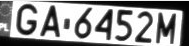
\includegraphics[width=\textwidth]{img/result-euro-input}
    \caption{Obraz wejściowy dla algorytmu segmentacji metodą szczytów histogramu}
    \label{fig:result_euro_input}
  \end{subfigure}
  ~
  \begin{subfigure}[b]{0.45\textwidth}
    
\includegraphics[width=\textwidth]{img/result-euro-bad}
    \caption{Obraz po procesie segmentacji, z~widocznym dodatkowym segmentem}
    \label{fig:result_euro_bad}
  \end{subfigure}
\begin{subfigure}[b]{0.45\textwidth}
    
\includegraphics[width=\textwidth]{img/result-euro-output}
    \caption{Obraz z~zaznaczonymi segmentami sklasyfikowanymi jako znaki}
    \label{fig:result_euro_output}
  \end{subfigure}
  \caption{Niepoprawna klasyfikacja segmentu jako znaku numeru rejestracyjnego}
  \label{fig:result_euro}
\end{figure}

\paragraph{Przerwy w~pojedynczym znaku}\mbox{} \\
Ten problem najczęściej występował dla metody rozrostu obszaru, ale pojawiał się również w~innych algorytmach segmentacji. Kiedy w~okolicach środka znaku jego wartości jasności przyjmują znacznie większe wartości (czyli obraz jest w~tym miejscu o~wiele jaśniejszy), algorytm może zaliczyć ten obszar jako tło, a~nie jako obraz. Dlatego może wystąpić efekt przerwy w~znaku, nie jest on ciągły. Z~punktu widzenia algorytmu są to tak naprawdę dwa segmenty, dlatego mogą one zostać odrzucone, lub zaklasyfikowane jako dwa osobne znaki (w zależności od tego, gdzie występuje wspominana wcześniej przerwa w~ciągłości). Rysunek~\ref{fig:result_przerwa} obrazuje ten problem. Można zauważyć, że litera $N$ zawiera przerwę, przez co została zrozumiana przez algorytm jako dwa znaki.

\begin{figure}
  \centering
  \begin{subfigure}[b]{0.45\textwidth}
    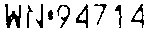
\includegraphics[width=\textwidth]{img/result-przerwa-bad}
    \caption{Obraz poddany procesowi segmentacji, zawierający przerwę w~jednej z~liter (litera N)}
    \label{fig:result_euro_input}
  \end{subfigure}
  ~
  \begin{subfigure}[b]{0.45\textwidth}
    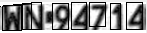
\includegraphics[width=\textwidth]{img/result-przerwa-output}
    \caption{Klasyfikacja segmentów - jeden ze znaków z~powodu przerwy, został rozpoznany jako dwa znaki}
    \label{fig:result_euro_bad}
  \end{subfigure}
  \caption{Problem przerw w~znakach }
  \label{fig:result_przerwa}
\end{figure}
